\chapter{Diversity Management for BFT Systems} 
\label{chap:lazarus_design}

This chapter presents the design of a control plane, named \system, to manage the diversity in \gls{bft} services.
The design improves the work presented in the previous chapters.
First, it adds new data and clustering techniques, introducing a new metric to evaluate vulnerabilities severity, and second, it proposes a strategy to minimize the risk of having common failure modes in replicated systems.
In the end, we validate this proposal against other strategies.

\section{Overview}
\system is a control plane solution that automatically changes the attack surface of a \gls{bft} system in a dependable way.
\system continuously collects security data from \gls{osint} feeds on the internet to build a knowledge base about the possible vulnerabilities, exploits, and patches related to the systems of interest.
This data is used to create clusters of similar vulnerabilities, which potentially can be affected by (variations of) the same exploit.
These clusters and other collected attributes are used to analyze the risk of the \gls{bft} system becoming compromised due to common vulnerabilities.
Once the risk increases, the control plane replaces a potentially vulnerable replica by another one, trying to maximize the failure independence of the replicated service.
Then, the replaced node is put on quarantine and updated with the available patches, to be re-used later.

\begin{figure}[t]
\begin{center}
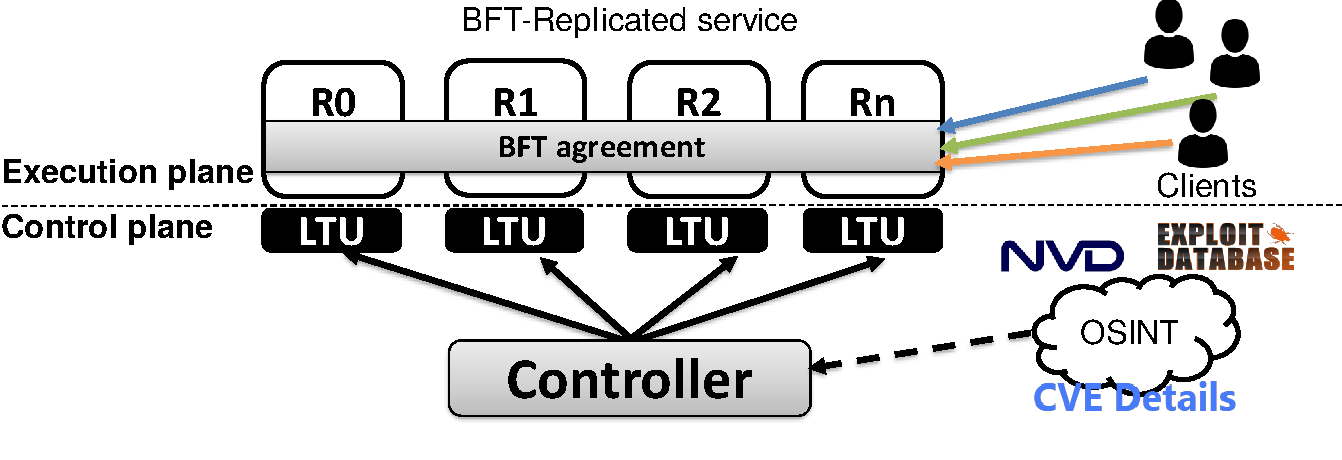
\includegraphics[width=0.7\columnwidth]{images/images/overview.pdf}
\caption{\system overview.}
\label{fig:overview}
\end{center}
\end{figure}

In a nutshell, as displayed in~Figure~\ref{fig:overview}, \system provides a distributed operating system for \gls{bft}-replicated services.
The system manages a set of nodes that run \emph{unmodified replicas} (encapsulated in \glspl{vm} or containers) in its execution plane. 
Each node must have a small \gls{ltu} that allows the activation and deactivation of replicas as demanded by the \system \emph{Controller}, in the control plane.
The controller decides which software should run at any given time by monitoring the vulnerabilities that potentially exist in the pool of replicas, aiming to minimize the risk of having several nodes being compromised by the same attack.



\section{System Model}
\label{sec:systemmodel}
\vspace{-4mm}
%\system system model shares some similarity with previous works on the proactive recovery of \gls{bft} systems~\cite{Castro:2002,Platania:2014,Sousa:2010,Roeder:2010}.
%More specifically, we consider a \emph{hybrid system model} composed of two planes (see Figure~\ref{fig:overview}) with different properties and assumptions:

\system system model shares some similarity with previous works on the proactive recovery of \gls{bft} systems~\cite{Castro:2002,Platania:2014,Sousa:2010,Roeder:2010,Distler:2011}.
More precisely, we consider a \emph{hybrid distributed system model} composed of two planes with different failure models:

\begin{itemize}

\item \textbf{Execution Plane:} replicas are subject to \emph{Byzantine failures} and communications go through an asynchronous network that can delay, drop or modify messages~\cite{Castro:1999,Kotla:2010,Bessani:2014,Aublin:2015}.
This plane hosts $n$ replicas from which at most $f$ can be compromised at any given moment.
In this chapter, we consider the typical scenario in which $n=3f+1$~\cite{Castro:2002,Kotla:2010,Aublin:2015}.  
\vspace{-2mm}
\item \textbf{Control Plane:}  
Each \emph{node} hosting a replica contains a \gls{ltu}, which is a fundamental trusted component~\cite{Sousa:2007} required for \emph{safe proactive recoveries}~\cite{Castro:2002,Sousa:2010,Roeder:2010,Platania:2014,Distler:2011}.
Each \gls{ltu} receives power on/off commands from a \emph{logically-centralized controller} to reconfigure their replicas.
As in previous works~\cite{Roeder:2010,Platania:2014,Sousa:2010}, this controller is assumed to be trusted.
Such assumption can be substantiated by running it in an isolated control network (similarly to cloud resource managers) our by building it in a trustworthy manner (tolerating Byzantine failures, as discussed in Section~\ref{sec:implementationdecisions}).

\end{itemize}


Besides the execution and control planes, we assume the existence of two types of external components: (1) clients of the replicated service, which can be subject to Byzantine failures; (2) \gls{osint} sources (e.g., \gls{nvd}, ExploitDB) that cannot be subverted and controlled by the adversary.
In practice, this assumption led us to consider only well-established and authenticated data sources.
Dealing with untrusted sources is an active area of research in the threat intelligence community (e.g.,~\cite{Sabottke:2015,Liu:2015}), which we consider out of the scope of this thesis.



%\section{Execution Plane}
%\label{sec:executionplane}

%The Execution Plane can accomodate any replicated system that already levareges on the existence of a controller node (e.g.,~\cite{Sousa:2010,Roeder:2010,Platania:2014,Garcia:2016}) or any \gls{bft} system that would benefit from the \system assistence (e.g.,~\cite{Sousa:2018}). 


%\section{Control Plane}
%\label{sec:controlplane}

%\system is the first control plane that automatically changes the attack surface of a \gls{bft} system in a dependable way.
%\system continuously collects security data from \gls{osint} feeds on the internet to build a knowledge base about the possible vulnerabilities, exploits, and patches related to the systems of interest.
%This data is used to create clusters of similar vulnerabilities, which potentially can be affected by (variations of) the same exploit.
%These clusters and other collected attributes are used to analyze the risk of the \gls{bft} system becoming compromised due to common vulnerabilities.
%Once the risk increases, \system replaces the potentially vulnerable replica by another one, trying to maximize the failure independence of the replicated service.
%Then, the replaced node is put on quarantine and updated with the available patches, to be re-used later.
%These mechanisms were implemented to be fully automated, removing the human from the loop.

%The current implementation of \system manages 17 \gls{os} versions, supporting the \gls{bft} replication of a set of representative applications.
%The replicas run in \glspl{vm}, allowing provisioning mechanisms to configure them. 
%We conducted two sets of experiments, one demonstrates that \system risk management can prevent a group of replicas from sharing vulnerabilities over time; the other, reveals the potential negative impact that virtualization and diversity can have on performance. 
%However, we also show that if naive configurations are avoided, \gls{bft} applications in diverse configurations can actually perform close to our homogeneous bare metal setup.

\section{Diversity of Replicas}
\label{sec:diversityofreplicas}

%BFT-replicated services running on \system are composed by $n$ replicas.
For our purposes, each \replica is composed of a stack of software, including an \gls{os} (kernel plus other software contained in an OS distribution), execution support (e.g., \gls{jvm}, \gls{dbms}), a \gls{bft} library, and the service that is provided by the system.
%(see Figure~\ref{fig:arch1}).
The set of $n$ replicas is called a \ES.

The fault independence of the replicas is improved when different \gls{ots} components are employed in the software stack~\cite{Deswarte:1998}. 
For example, it has been shown that using distinct databases~\cite{Gashi:2007}, \glspl{os}~\cite{Garcia:2013}, and filesystems~\cite{Castro:2003,Bairavasundaram:2009}, can yield important benefits in terms of fault independence. 
In addition, automatic techniques could enhance diversity, like randomization/obfuscation of \glspl{os}~\cite{Roeder:2010}, applications~\cite{King:2016}, and \gls{bft} libraries~\cite{Platania:2014}.
Although \system can also exploit these automatic techniques, in this chapter we center our attention on diverse \gls{ots} components. 
In particular, \system monitors the disclosed vulnerabilities of all elements of the replicas' software stacks to assess which of them may contain common vulnerabilities.  

In the experimental evaluation, however, we focus on the diversity of \glspl{os} (\emph{not only their kernel}, but the whole \gls{os} distribution) because: (i) by far, most of the replica's code is the \gls{os}; 
(ii) such size and the role played in the stack, makes the \gls{os} a significant target, with new vulnerabilities and exploits being discovered every day; 
and (iii) there are many alternative \glspl{os} to bring variety. 
The two last factors are particularly important to enrich the validity of our analysis. 
Consequently, we will not explicitly consider the diversity of the \gls{bft} library (i.e., the protocol implementation) or the service code implemented on top of it. 
Three arguments justify this decision: (1) N-version programming is too costly~\cite{Avizienis:1977}; (2) the small size of such components\footnote{For example, a BFT key-value store based on BFT-SMaRt has less than 15k lines of code in total~\cite{Bessani:2014}.} makes them relatively simpler to test and assess with some confidence~\cite{Martins:2013,Lee:2014}; and (3) a few works show that such protocol implementations can be generated from formally verified specifications, resulting in no vulnerabilities at this level~\cite{Hawblitzel:2015,Rahli:2018};
Notice that, although we do not explicitly consider the diversity of \gls{bft} libraries, nothing prevents \system from monitoring them in a similar way as the \glspl{os}.
However, there are no reported vulnerabilities about these to support our study.
%Additionally, if this is a concern, automatic diversity techniques could be added to this layer~\cite{Platania:2014,Roeder:2010}.


\section{Diversity-aware Reconfigurations}
\label{sec:metric}

One of the goals of this thesis is to maintain the fault independence of the running \ES given the present knowledge about vulnerabilities.
The core of this chapter is the \emph{vulnerability evaluation method} used to assess the risk of having replicas with shared vulnerabilities, and an algorithm to trigger replacements when necessary.

\subsection{Finding Common Vulnerabilities}
\label{sec:common_vulnerabilities}

%\gls{nist}'s \gls{nvd}~\cite{nvd} is the authoritative data source for disclosure of vulnerabilities and associated information~\cite{Massacci:2010}. 
%\gls{nvd} aggregates vulnerability reports from more than 70 security companies, advisory groups, and organizations, thus being the most extensive vulnerability database on the web. 
%All data is made available as \gls{xml} data feeds, containing the reported vulnerabilities on a given period. 
%Each \gls{nvd} vulnerability receives a unique identifier and a short description provided by the \gls{cve}~\cite{cveterm}. 
%The \gls{cpe}~\cite{cpe} provides the list of products affected by the vulnerability and the date of the vulnerability publication.
%The \gls{cvss}~\cite{cvss} calculates the vulnerability severity considering several attributes, such as the attack vector, privileges required, exploitability score, and the security properties compromised by the vulnerability (i.e., integrity, confidentiality, or availability).
%WE USE THE NVD (as described in Chapter~\ref{chap:datasource}

\begin{table}[!t]
\begin{center}
{\small
\begin{tabular}{| p{2.8cm} | p{10.0cm} | }\hline
\textbf{CVE (affected OS)} & \textbf{Description} \\\hline\hline
CVE-2014-0157 (Opensuse 13) & \small \gls{xss} vulnerability in the Horizon Orchestration dashboard in OpenStack Dashboard (aka Horizon) 2013.2 before 2013.2.4 and icehouse before icehouse-rc2 allows remote attackers to inject arbitrary web script or HTML via the description field of a Heat template. \\ \hline
CVE-2015-3988 (Solaris 11.2) & \small Multiple \gls{xss} vulnerabilities in OpenStack Dashboard (Horizon) 2015.1.0 allow remote authenticated users to inject arbitrary web script or HTML via the metadata to a (1) Glance image, (2) Nova flavor or (3) Host Aggregate. \\ \hline
CVE-2016-4428 (Debian 8.0) & \small \gls{xss} vulnerability in OpenStack Dashboard (Horizon) 8.0.1 and earlier and 9.0.0 through 9.0.1 allows remote authenticated users to inject arbitrary web script or HTML by injecting an AngularJS template in a dashboard form. \\ \hline
\end{tabular}
}
\vspace{2mm}
\caption{Similar vulnerabilities affecting different OSes.}
\label{tab:missing_products}
\end{center}
\end{table}

The first step of our method is to query vulnerability databases on the internet to find the common vulnerabilities that may affect the \gls{bft} system.

Previous studies on diversity count the \gls{cve} entries that list multiple \glspl{os}, as they should represent vulnerabilities that are shared, assuming that less common vulnerabilities imply a smaller probability of compromising $f+1$ replicas~\cite{Garcia:2013}.
Although this intuition may seem acceptable, in practice it underestimates the number of vulnerabilities that compromise two or more OSes due to imprecisions in the data source. 
For example, Table~\ref{tab:missing_products} shows three vulnerabilities, affecting three different OSes at distinct dates.
At first glance, one may consider that these \glspl{os} do not have the same vulnerability.
However, a careful inspection of the descriptions shows that they are very similar.
Moreover, we checked this resemblance by searching for additional information on security web sites, and we found out that CVE-2016-4428, for example, also affects Solaris.\footnote{\url{https://www.oracle.com/technetwork/topics/security/bulletinjul2016-3090568.html}}

Even with these imperfections, \gls{nvd} is still the best data source for vulnerabilities.
Therefore, we exploit its curated data feeds for obtaining the unstructured information present in the vulnerability text descriptions and use this information to find similar weaknesses.
A usual way to find similarity in unstructured data is to use clustering algorithms~\cite{Jain:2010}.
Clustering is the process of aggregating related elements into groups, named clusters, and is one of the most popular unsupervised machine learning techniques. 
We apply this technique to build clusters of similar vulnerabilities (see Chapter~\ref{chap:lazarus_implementation} for details), even if the data feed reports that they affect different products.
For example, the vulnerabilities in Table~\ref{tab:missing_products} will be placed in the same cluster as there is a significant resemblance among the descriptions, and they can potentially be activated by (variations of) the same exploit.


\subsection{Measuring Risk}
\label{sec:measurerisk}


\begin{table}[t]
\begin{center}
{\small
\begin{tabular}{| c | c | }\hline
\textbf{Rating} & \textbf{CVSS Score} \\\hline\hline
\texttt{NONE} & 0.0 \\
\texttt{LOW} & 0.1-3.9 \\
\texttt{MEDIUM} & 4.0-6.9 \\
\texttt{HIGH} & 7.0-8.9 \\
\texttt{CRITICAL} & 9.0-10.0 \\ \hline
\end{tabular}
}
\vspace{2mm}
\caption{Qualititative CVSS severity rating scale.}
\label{tab:cvss_scale}
\end{center}
\end{table}

Once the set of common vulnerabilities is found, our method assigns a score to each vulnerability in the set.

As presented in Chapter~\ref{chap:datasource}, each vulnerability in NVD has associated a few \gls{cvss} severity scores and metrics~\cite{cvssv3}.
The scores provide a way to marshal several vulnerability attributes in a value reflecting various aspects that impact security. 
The score value can also be translated into a qualitative representation to assist on the vulnerability management process, i.e., from \texttt{NONE} ($0.0$) to \texttt{CRITICAL} ($9.0$ to $10.0$) as presented in Table~\ref{tab:cvss_scale}.

\gls{cvss} has some limitations that can make it inappropriate for managing the risk associated with a replicated system:
(1) there is no correlation between the \gls{cvss} exploitability score and the availability of exploits in the wild for the vulnerability~\cite{Bozorgi:2010}; 
(2) \gls{cvss} does not provide information about the date when a vulnerability starts to be exploited and when the patch becomes ready; 
and (3) \gls{cvss} does not account for the vulnerability age, which means that severity remains the same over the years~\cite{Frei:2006}; 
therefore, a very old vulnerability can end up being considered as critical as a recent one, even though for the former there has been plenty of time to update the component and/or the defenses.  


Given these shortcomings, we propose a \gls{cvss} extension and use it to measure the risk of a \gls{bft} system configuration having replicas with shared vulnerabilities.
This extension is mostly focused on differentiating vulnerabilities by their current \emph{potential exploitability}, aiming to surpass the limitations identified above.
In this process, (1) and (2) are addressed by using additional \gls{osint} sources (e.g., other security databases and vendor sites) that provide information about exploits and dates. 
In fact, often vendor sites also give additional product versions compromised by the vulnerability, thus improving the accuracy of the analysis. 
Limitation (3) is settled by decreasing the criticality of a vulnerability gradually through time.

Our \gls{cvss} extension uses four factors that together contribute to the overall score. 
The starting factor is the \gls{cvss} core score, as it is a good basis that takes into consideration several attributes of the vulnerability.
The other three factors adjust the score taking into account the age and the availability of a patch and an exploit. 
The rationale is to allow the ranking of vulnerabilities according to their possible exploitation at a given moment in time.
The worst scenario (higher severity score) corresponds to a vulnerability that is new (N) (i.e., recently published), for which there is an exploit already being distributed (E), and that is not yet patched -- called NE.
The best scenario (lowest score) is when a vulnerability is old (O) and there is a patch (P), and apparently, no viable exploit has been crafted -- named OP. 
Between the two extremes, several cases of vulnerabilities are considered, with their scores calculated accordingly (see Figure~\ref{fig:scale}).



\begin{figure}[!t]
\begin{center}
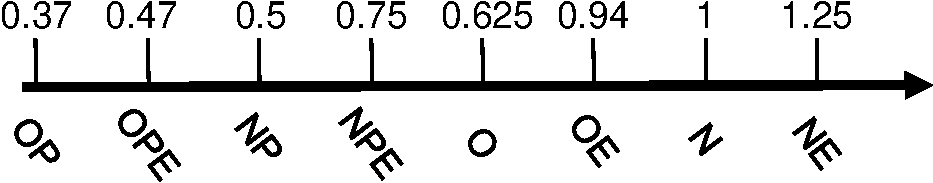
\includegraphics[width=0.7\columnwidth]{images/images/scale.pdf}
\caption{Scoring system of vulnerabilities based on age, patch, and exploit.}
\label{fig:scale}
\end{center}
\end{figure}


The metric is defined in Equation~\ref{eq:score}.
It is a multiplication of the \gls{cvss} core score~\cite{cvssv3} by three adjusting factors. 
The first is \emph{Oldness}, which causes criticality to decrease over time. 
It is harmonized by the \emph{Oldness Threshold} and the interval\footnote{\textit{Oldness Threshold} is set to 365 in our calculations; \textit{now()} and $v_i.published\_date$ return the current day and the day when the vulnerability was published, respectively.} that has passed since the vulnerability publication (Equation~\ref{eq:oldness}). 
In addition, this factor is bounded by a minimum value that impedes it from reaching zero (which would cause the vulnerability to be left unnoticed).
The second is \emph{Patched}, which reduces the severity by half when a patch is available (Equation~\ref{eq:patched}; $v_{i}.patched$ is an on/off flag).
Finally, the \emph{Exploited} factor grows severity by a quarter when an exploit is made available (Equation~\ref{eq:exploited}; $v_{i}.exploited$ is again a on/off flag).
The constants in these equations were defined to ensure the aggregated modifiers correspond to Figure~\ref{fig:scale}.
%In the end our modified vulnerability score ranges from $0.0$ to $12.5$.
\begin{equation}
\begin{split}
\text{score(v$_i$)}=\text{CVSS(v$_i$)}\times\text{oldness(v$_i$)}\times\text{patched(v$_i$)}\times\text{exploited(v$_i$)}
\label{eq:score}
\end{split}
\end{equation}
\begin{equation} 
\begin{split}
\text{oldness(v$_i$)}=\text{max}\left((1-0.25\times\frac{(\text{now()}-\text{v$_i$.published\_date)}}{\text{Oldness Threshold}}), 0.75\right)
\label{eq:oldness}
\end{split}
\end{equation}
\begin{equation} 
\text{patched(v$_i$)}=0.5^{\text{v$_i$.patched}}
\label{eq:patched}
\end{equation} 
\begin{equation}
\text{exploited(v$_i$)} = 1.25^{\text{v$_i$.exploited}}
\label{eq:exploited}
\end{equation}  


Figure~\ref{fig:scoreplot} displays our score and \gls{cvss} for three example vulnerabilities:
(a) NE is a vulnerability that is new and has no patch yet, but an exploit was made available a few days after publication. 
Our score starts by decaying slowly but then there is a jump on severity when the exploit is published;
(b) OP represents the best scenario, where the vulnerability is \emph{old} and a patch was eventually distributed (and no exploit is available). 
Here, the severity decreases once there is a patch, losing its relevance over time from a security perspective; 
and (c) NPE illustrates a vulnerability that has an exploit a few days after publishing and then a patch is also created.
First, the score is raised once the exploit starts to be distributed, next it decreases three days later after the patch is released, and then continues to decay over time.


\begin{figure}[!t]
\subfloat[CVE-2018-8303.]{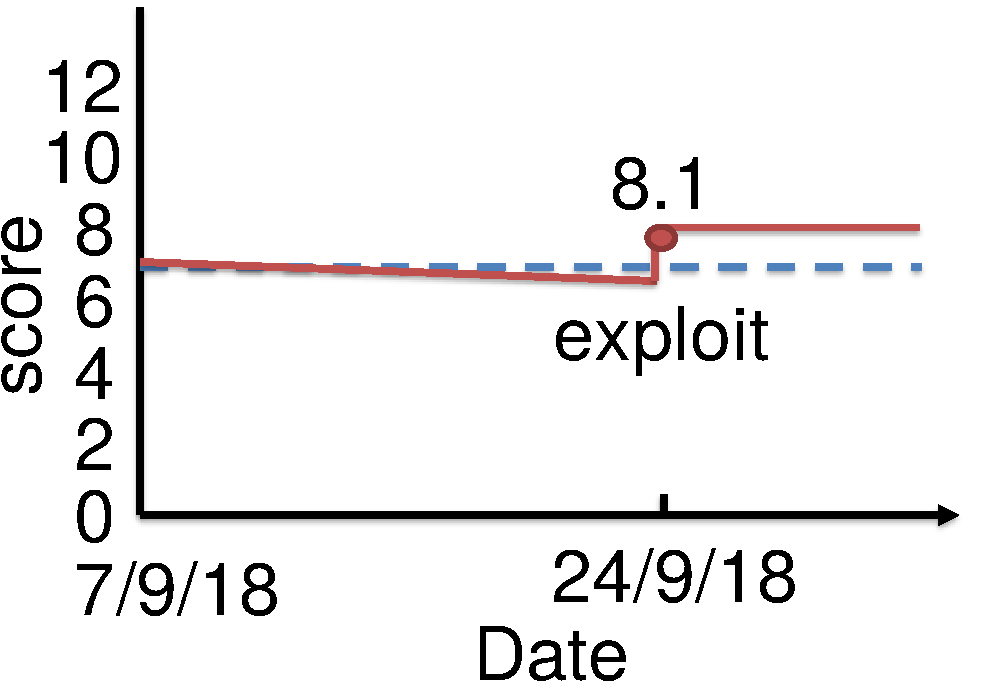
\includegraphics[width=0.32\columnwidth]{images/images/NE.pdf}\label{fig:ne}} %for Windows 10
\subfloat[CVE-2016-7180.]{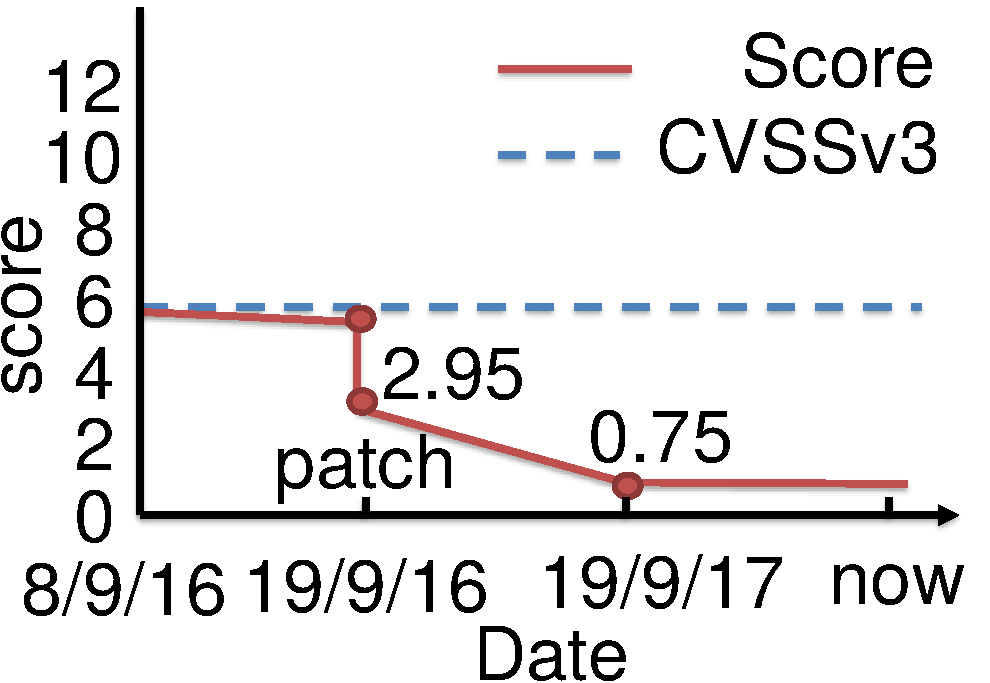
\includegraphics[width=0.32\columnwidth]{images/images/OP.pdf}\label{fig:op}}%Debian 9.0
\subfloat[CVE-2018-8012.]{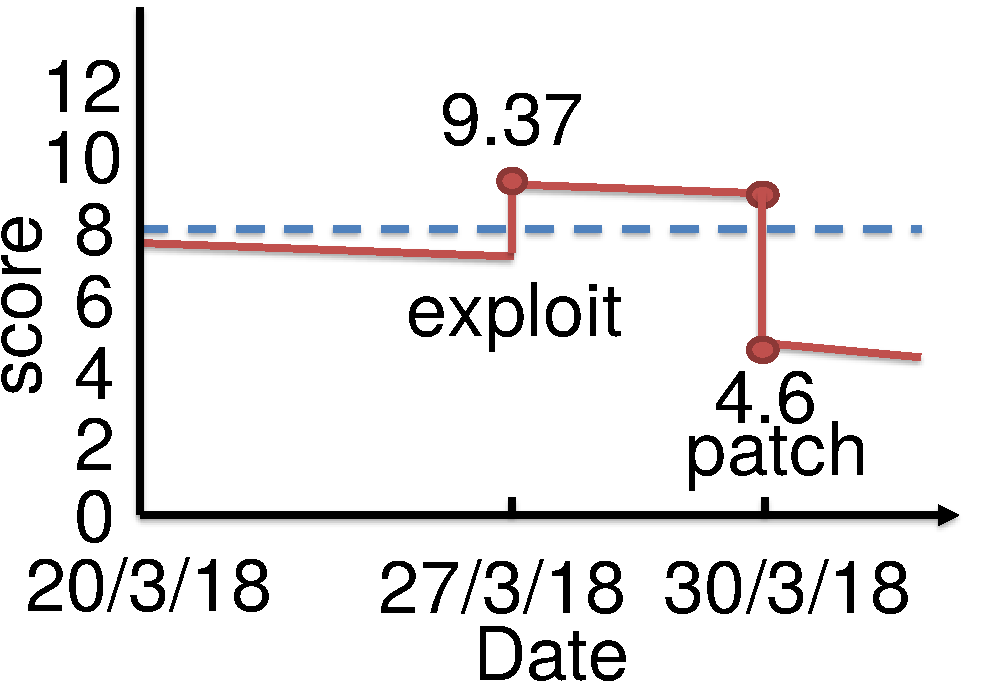
\includegraphics[width=0.32\columnwidth]{images/images/NPE.pdf}\label{fig:npe}} %Debian 9.0
\caption{\footnotesize{Examples of \emph{score(v$_i$)} for three vulnerabilities.}}
\label{fig:scoreplot}
\end{figure}



\subsection{Measuring Configurations Risk}
\label{sec:risk}

%After discovering common vulnerabilities and assigning a dynamic score to them, the third step of our method is to calculate the \emph{risk of a set of replicas} to be compromised in the current threat landscape.

The third step of our method is to calculate the \emph{risk of a set of replicas} according to the score of the common weaknesses.
The risk associated with a \ES with $n$ replicas is given by Equation~\ref{eq:risk}. 
It sums up the score (Equation~\ref{eq:score}) of the vulnerabilities that would allow an attack to compromise simultaneously a pair of replicas $r_i,r_j \in \ES$.
%Function \emph{common()} employs our score, as it aggregates security features of a vulnerability, and other information collected from OSINT sources. To begin, the function gathers all the vulnerabilities that would allow an attack to compromise simultaneously a pair of replicas ($rc_i,rc_j$). 
More precisely, the vulnerabilities in $\mathcal{V}(r_i,r_j)$ aggregate: (i) the vulnerabilities that affect the software running in both replicas as listed in \gls{nvd} (and other \gls{osint} sites); and (ii) groups of vulnerabilities that are placed in the same cluster and affect each replica in the pair (as explained in Section~\ref{sec:common_vulnerabilities}). 
%The final score is normalized with function \emph{norm()} to generate a value between 0 and 1.
%Next, the function calculates the score of each vulnerability, and returns the sum of all scores. 
%The risk metric computes \emph{common()} for all combinations of replica pairs in the configuration and accumulates the values. 

\begin{equation}
\mathit{risk(\ES)}=\sum_{r_i,r_j \in \ES}^{} \hspace{1.2mm} \sum_{v \in \mathcal{V}(r_i,r_j)}^{}\mathit{score(v)}
\label{eq:risk}
\end{equation} 

This metric penalizes configurations that include replica pairs containing more common weaknesses, as this is an indication that they are less fault-independent.
In addition, the level of penalty is kept proportional to the severity of these vulnerabilities as observed at the time of the calculation. 
For example, replicas that share weaknesses only in the distant past are considered less risky than replicas with recently highly exploitable common vulnerabilities.


\subsection{Selecting Configurations}
\label{sec:configurations}

The final step of our method is to periodically assess the risk of a deployed configuration and its future replacement of replicas according to the score evaluation of our metric.


Algorithm \ref{alg:algorithm2} details the procedure that is taken to select the running \ES.
%This is done by periodically evaluating the risk of the current \ES. 
If its risk exceeds a predefined \emph{threshold}, a mechanism is triggered to replace replicas and reduce the overall risk.
When this happens, the algorithm picks a new replica from the available candidates (\RS) to join \ES. 
In addition, it removes the replica that reduces the overall risk and sets it aside (i.e., in \QS) to impede its re-selection.
There, the replicas wait for patches before they re-join \RS and become ready to be chosen again.
Moreover, the algorithm ensures that the running replicas will eventually be replaced, despite their overall score.


Function \emph{Monitor()} (line 5) is called on each monitoring round (e.g., at midnight every day) to evaluate the current configuration.
%Consider a \ES that is already running with a risk$=\alpha$.
If the risk of \ES is greater or equal than a certain \emph{threshold} (line 6), the algorithm will assess which replica should be replaced.
First, it initializes two variables, the candidates list (line 7) and all possible combinations of $n-1$ out of $n$ elements of \ES (line 8).
Then, each element \texttt{r} in \RS (line 9) is tested as a potential substitute, i.e., as the $n^{th}$ element that would complete each of the combinations \COMB with $n-1$ replicas (line 10).
Next, we define a \ES' as the union of \COMB and $r$ (line 11).
The risk of \ES' is calculated (line 12) and added to a list that stores the tuple $\langle$\ES', \texttt{score}$\rangle$ (line 13). 
At the end of the these nested loops, we have a list with all the possible combinations of \ES and \RS together with their risk.
Then, the function \Rand selects a configuration randomly from the list of candidates (line 14). 
Although it is not present in the algorithm, it only selects configurations which are below the \emph{threshold} score. 
Then the algorithm updates all the sets (line 15) using the function \Replace (lines 36-40). 
To decide which element needs to be removed from \ES it makes the difference between the current \ES and \SC (line 37) and the contrary to select the element to join the \ES (line 38).
Then, \toRemove is added to \QS (line 39), removed from \ES and the new element is added to the \ES (line 40).
 
If the risk of \ES is lower than the \emph{threshold} (line 16), the algorithm assess if a reconfiguration is needed.
In this scenario, we start by initializing the variable \toRemove as empty (line 17) and \texttt{maxScore} with the value of the CVSS score rating \texttt{HIGH} (line 18).
For each element of \ES (line 19) the algorithm calculates the average score of the vulnerabilities affecting \r using Equation~\ref{eq:score} (line 20).
Then, if the average vulnerability score is equals or greater than \texttt{HIGH} (line 21), the variable \toRemove is set to the element \r (line 22) and the value of \texttt{maxScore} with the \texttt{avgScore} (line 23).
At the end of the loop, the algorithm knows which is the element \r from \ES that has vulnerabilities with a highest average score.
If \toRemove is empty, the algorithm proceeds to line 32. 
Otherwise, there is an element that is a candidate to leave \ES and a new replica, that improves the overall score will be selected (line 24).
First, the \texttt{candidate\_list} is set as empty (line 25).
Next, for each element \r' in \RS (line 26) the algorithm tests a \ES' with \r' instead of \toRemove (line 27).
Then, the score for this configuration is calculated (line 28) and together with the \ES' is stored in a list of candidates (line 29).
As already described, the function \Replace updates the elements of the sets (line 31).


{\centering
\begin{minipage}{.8\linewidth}
\small
\begin{algorithm}[H]
%\begin{multicols}{2}
%\SetInd{0.3em}{0.2em}
\setstretch{1.0}
\caption{Replica Set Reconfiguration}\label{alg:algorithm2}
{\small
\ES: set replicas executing \;
$n$: number of replicas in \ES\;
\RS: set with the available replicas (not in use)\;
\QS: set of quarantine replicas\;
\BlankLine
\Fn{Monitor()}{
	\If{\Risk{\ES} $\geq$ threshold}{	
		\texttt{cadidates\_list} $\leftarrow$ $\perp$\;
		\COMBS = ${n\choose n-1}$\ES\;
		\ForEach{$ r $ in \RS}{
			\ForEach{$ \COMB $ in \COMBS}{
				\ES' $\leftarrow$ \COMB $\cup$ \{r\}\;
				\texttt{score} $\leftarrow$ \Risk{\ES'}\;
				\texttt{cadidates\_list}.add($\langle$\ES', \texttt{score}$\rangle$)\;
			}
		}
	\SC $\leftarrow$ \Rand{\texttt{cadidates\_list}} \;
	\Replace{\SC}\;		
	}
    \Else{
		\toRemove $\leftarrow$ $\perp$\;
		\texttt{maxScore} $\leftarrow$ \texttt{HIGH}\;
		\ForEach{$ r $ in \ES}{
			\texttt{avgScore} $\leftarrow$ \oldestVulnerability{r}\;
			\If{ avgScore $\geq$ maxScore}{	
				\toRemove $\leftarrow$ $r$\;
				\texttt{maxScore} $\leftarrow$ avgScore\;
			}
	}
		\If{ \toRemove $\neq$ $\perp$}{
			\texttt{cadidates\_list} $\leftarrow$ $\perp$\;				
			\ForEach{$ r' $ in \RS}{
				\ES' $\leftarrow$ (\ES $\setminus$ \{toRemove\}) $\cup$ \{r'\}\;
				%\ES' $\leftarrow$ \ES' $\cup$ \{r'\}\;
				\texttt{score} $\leftarrow$ \Risk{\ES'}\;	
				\texttt{cadidates\_list}.add($\langle$\ES', \texttt{score}$\rangle$) \;
			}
			\SC $\leftarrow$ \Rand{\texttt{cadidates\_list}} \;
			\Replace{\SC}\;
		}
	}
	\ForEach{$ r $ in \QS}{	
		\If{\patched{r} = TRUE}{	
			\QS $\leftarrow$ \QS $\setminus$ $\{r\}$\;
			\RS $\leftarrow$ \RS $\cup$ $\{r\}$\;
		}
	}
}
\Fn{updateSets(\SC)}{
		\toRemove $\leftarrow$ $x \in (\ES \setminus \SC)$\;
		\toJoin $\leftarrow$ $y \in (\SC \setminus \ES)$\;
		\QS $\leftarrow$ \QS $\cup$ $\{toRemove\}$\;
		\ES $\leftarrow$ (\ES $\setminus$ $\{toRemove\}$) $\cup$ $\{toJoin\}$\;

}
}
\end{algorithm}
\end{minipage}
\par
}

Finally, the \RS and \QS are updated.
Each \QS element (line 32) is checked if it is fully patched (line 33).
In the affirmative case, the element is removed from \QS (line 34) and added to the \RS again (line 35).
We did not present two unlikely corner cases where a \emph{system admin} may need to intervene: if the \RS runs out of elements or \emph{rand()} cannot return a configuration that minimizes the risk of the system.
We propose at least two actions to preserve availability under some risk of becoming compromised: increase the \emph{threshold} or removing the elements with fewer unpatched vulnerabilities from \QS to \RS.

\section{Evaluation}
\label{sec:diversity}


This section evaluates how our method performs on the selection of dependable replica configurations.
As discussed in Section~\ref{sec:diversityofreplicas}, we focus our experimental evaluation solely on the \gls{os} diversity.
In particular, we considered 21 \gls{os} versions 
% to be deployed on four replicas with 
of the following distributions: OpenBSD, FreeBSD, Solaris, Windows, Ubuntu, Debian, Fedora, and Redhat. 

These experiments emulate live executions of the system by dividing the collected data into two periods.
The goal is to create a knowledge base in a \emph{learning phase} that is used to assess \system' choices during an \emph{execution phase}.
(1) The \emph{learning phase} comprises all vulnerabilities between \emph{2014-1-1} and the beginning of the \emph{execution phase}; 
and (2) the \emph{execution phase} is divided into monthly intervals, from January to August of 2018, allowing for eight independent tests. 
%This last period is divided into monthly intervals allowing for eight independent tests.
%For example, to run the experiment in May the \emph{learning phase} starts on \emph{2014-1-1} and ends on \emph{2018-4-30}, then the \emph{execution phase} starts on the May $1^{st}$ until the end of the month. 
A run starts on the first day of the \emph{execution phase} and then progresses through each day until the end of the interval. 
Every day, we check if the executing replica set could be compromised by an attack exploring the vulnerabilities that were published in that month. 
We take the most pessimistic approach, which is to consider the system as broken if a single vulnerability comes out affecting at least two \glspl{os} executing at that time.
Therefore, if one of the \glspl{os} already has a patch for the tested vulnerability, it is not counted as compromised.


Four additional strategies, inspired by previous works, were defined to be compared with \system (Section~\ref{sec:configurations}):

\begin{itemize}

\item \textbf{Equal:} all the replicas use the same randomly-selected \gls{os} during the whole execution. 
This corresponds to the scenario where most past \gls{bft} systems have been implemented and evaluated (e.g.,~\cite{Kotla:2010,Aublin:2015,Behl:2015,Veronese:2013,Behl:2017,Liu:2016,Yin:2003,Amir:2011,Bessani:2014,Clement:2009b}). 
Here, compromising a replica would mean an opportunity to intrude the remaining ones.

\item \textbf{Random:} a configuration of $n$ \glspl{os} is randomly selected, and then a new \gls{os} is randomly picked to replace an existing one each day. 
This solution represents a system with proactive recovery and diversity, but with no informed strategy for choosing the next \ES.

\item \textbf{Common:} this strategy is the straw man solution to prevent the existence of shared vulnerabilities among \gls{os}. 
This strategy minimizes the number of common vulnerabilities for each set and was introduced in previous vulnerability studies~\cite{Garcia:2012}.

\item \textbf{CVSS v3:} this strategy is very similar to ours as it tries different combinations to find the best one that minimizes the sum of \gls{cvss} v3 score.


\end{itemize}


\subsection{Diversity vs Vulnerabilities}

We evaluate how each strategy can prevent the replicated system from being compromised. 
Each strategy is analyzed over $1000$ runs throughout the execution phase in monthly slots. 
Different runs are initiated with distinct random number generator seeds, resulting in potentially different OS selections over time. 
On each day, we check if there is a vulnerability affecting more than one replica in the current \ES, and in the affirmative case the run is stopped.


\begin{figure}[t]
\begin{center}
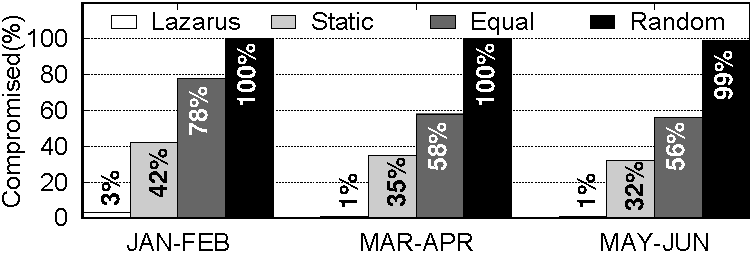
\includegraphics[width=\columnwidth]{images/gnuplot/executions/execution.pdf}
\caption{Compromised system runs over eight months.}
\label{fig:all_vulns}
\end{center}
\end{figure}


\textbf{Results:} Figure~\ref{fig:all_vulns} compares the percentage of compromised runs of all strategies. 
Each bar represents the percentage of runs that did not terminate successfully (lower is better). 
\system presents the best results for every month.
The \emph{Random} and \emph{Equal} strategies perform worse because eventually, they pick a group of OSes with common vulnerabilities as they do not make decisions with specific criteria. 
Although some criteria guide the other strategies, most of them present a majority of executions compromised during the experiments.
This result provides evidence for the claim that \system improves the dependability, reducing the probability that $f+1$ OSes eventually become compromised and contrary to intuition, changing OSes every day with no criteria will always create unsafe configurations.


Nonetheless, the results from May deserve a more careful inspection. 
We have identified some CVEs that make it very difficult to survive to common vulnerabilities even using the \system strategy.
For example, CVE-2018-1125 and CVE-2018-8897 affect a few Ubuntu and Debian releases simultaneously.
There are also a set of vulnerabilities affecting several Windows releases (e.g., CVE-2018-8134 and CVE-2018-0959). 
We also found a vulnerability (CVE-2018-1111) that affects few Fedora releases and one Redhat release. 

\subsection{Diversity vs Attacks}


This experiment evaluates the same strategies when facing notable attacks that appeared in 2017. 
Each attack potentially exploits several flaws, some of which affecting different OSes. 
The attacks were selected by searching the security news sites for high impact problems, most of them related to more than one CVE. 
As some of the CVEs include applications, we added more vulnerabilities to the database for this purpose. 
We have considered the following attacks:
WannaCry~\cite{wannacry}, Stackclash~\cite{stacklash}, and Petya~\cite{petya}.
Table~\ref{tab:attacks} provides a summary of these attacks.



Since some of these attacks might have been prepared months before the vulnerabilities are publicly disclosed, we augmented the execution phase to the full eight months. 
Therefore, we set \emph{learning phase} to begin \emph{2014-1-1} and to end on \emph{2017-12-31}. 
The \emph{execution phase} period that starts on 2018 January and finishes on August 2018. 
As before, the strategies are executed over $1000$ runs. 


\begin{table}[t]
\begin{center}
{%\small%
\small
\begin{tabular}{ | c | p{0.80\columnwidth} | }\hline
\textbf{Attack name}  & \textbf{Attack Summary}\\ \hline

\textbf{Wanna Cry} & \emph{On Friday, May 12, 2017, the world was alarmed to discover a widespread ransomware attack that hit organizations in more than 100 countries. Based on a vulnerability in Windows' SMB protocol (nicknamed EternalBlue), discovered by the NSA and leaked by Shadow Brokers.}
\\ \hline

\textbf{Stackclash} & \emph{In its 2017 malware forecast, SophosLabs warned that attackers would increasingly target Linux. The flaw, discovered by researchers at Qualys, is in the memory management of several operating systems and affects Linux, OpenBSD, NetBSD, FreeBSD and Solaris.}
\\ \hline

\textbf{Petya} & \emph{A new strain of the Petya ransomware started propagating on June 27, 2017, infecting many organizations. Petya uses the EternalBlue exploit as one of the means to propagate itself. However, it also uses classic SMB network spreading techniques, meaning that it can spread within organizations, even if they have patched against EternalBlue.}
\\ \hline


\end{tabular}
}
\vspace{2mm}
\caption{Notable attacks during 2017.}
\label{tab:attacks}
\end{center}
\end{table}

\begin{figure}[t]
\begin{center}
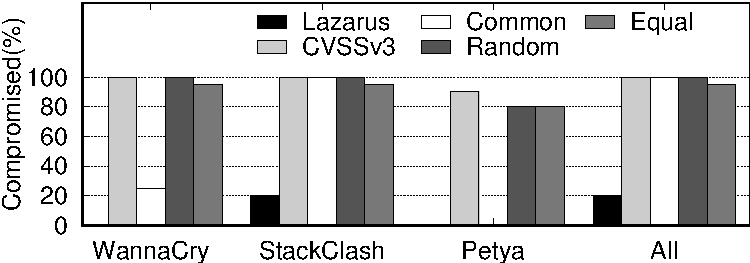
\includegraphics[width=\columnwidth]{images/gnuplot/attacks/attacks.pdf}
\caption{Compromised runs with notable attacks.}
\label{fig:special_vulns}
\end{center}
\end{figure}
\vspace{-1mm}


\textbf{Results:}
Figure~\ref{fig:special_vulns} shows the percentage of compromised runs for each attack and all attacks put together.
\system is the best at handling the various scenarios, with almost no compromised executions.
The StackClash is the most destructive attack as it is the one affecting more \glspl{os}.
Therefore, decisions guided by a criteria that aim to avoid common vulnerabilities may also fail. 
Nevertheless, the results show that such strategies do improve the resilience to attacks.




\section{Final Remarks}
\label{sec:finalremarkslazarusdesign}

\system addresses the long-standing open problem of evaluating, selecting, and managing the diversity of a \gls{bft} system to make it resilient to malicious adversaries.
This chapter shows an approach to select the best replicas to run together given the current threat landscape and evaluate the proposed strategy.
In the next chapter, we discuss how this strategy can be implemented and the overhead of using \gls{os} diversity.

